\textbf{Приклад задачі відновлення ваг.}\\
\begin{figure}[H]
    \centering
    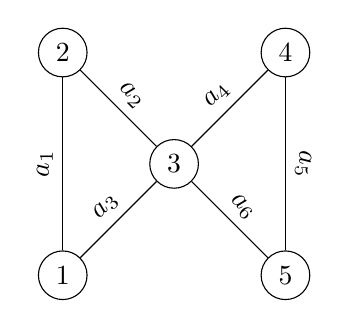
\begin{tikzpicture}[node distance={20mm}, main/.style = {draw, circle}]
    \node[main] (1) {$2$}; 
    \node[main] (2)[below right of=1] {$3$};
    \node[main] (3)[above right of=2] {$4$};
    \node[main] (4)[below right of=2] {$5$};
    \node[main] (5)[below left of=2] {$1$};
    \draw (1) -- node [ above, midway, sloped] {$a_2$}(2);
    \draw (2) -- node [ above, midway, sloped] {$a_4$}(3);
    \draw (3) -- node [ above, midway, sloped] {$a_5$}(4);
    \draw (4) -- node [ above, midway, sloped] {$a_6$}(2);
    \draw (2) -- node [ above, midway, sloped] {$a_3$}(5);
    \draw (5) -- node [ above, midway, sloped] {$a_1$}(1);
    \end{tikzpicture}\\
    \caption{$\bf G$ - граф метелик}
    \label{zad:image}
\end{figure}
\textit{Умова}: Нехай нам відомий граф G зображений на рисунку \ref{zad:image}. Необхідно відновити усі ваги  за спектром вихідного графа, і спектром його підграфів: ребер (4,5) і (2,3), ${\bf G}-\{5\}$.\\
$\sigma({\bf G}) = \{-6.91, -4.406, -0.962, 1.75,10.528\}$\\
$\sigma((4,5)) = \{-5,5\}$\\
$\sigma((2,3)) = \{-2,2\}$\\
$\sigma({\bf G}-\{5\}) = \{-5.206, -0.977, 0.559, 5.624\}$

\textit{Розв'язання}

1. Відновимо характеристичні многочлени з відомих за умовою спектрів.\\
$P_{\bf G}(\lambda) = (\lambda + 6.91)(\lambda + 4.406)(\lambda + 0.962)(\lambda - 1.75)(\lambda - 10.528) = \lambda^5-91\lambda^3-252\lambda^2+402\lambda+540$\\
$P_{(4,5)}(\lambda) = (\lambda + 5)(\lambda - 5) = \lambda^2 - 25$\\
$P_{(2,3)}(\lambda) = (\lambda + 2)(\lambda - 2) = \lambda^2 - 4$\\
$P_{\bf G-\{5\}}(\lambda) = (\lambda + 5.206)(\lambda + 0.977)(\lambda - 0.559)(\lambda - 5.624) = \lambda^4-30\lambda^2-12\lambda+16$

2. Випишемо характеристичні многочлени у загальному вигляді, де коефіцієнти невідомі.
\begin{multline*}
P_{\bf G}(\lambda) = \lambda^5 - (a_1^2+a_2^2+a_3^2+a_4^2+a_5^2+a_6^2)\lambda^3 - 2\lambda^2(a_1a_2a_3 + a_4a_5a_6) + \\
+(a_1^2a_4^2+a_1^2a_5^2+a_2^2a_5^2+a_3^2a_5^2+a_1^2a_6^2)\lambda
+2(a_1a_2a_3a_5^2 +a_4a_5a_6a_1^2)
\end{multline*}
$P_{\bf G-\{5\}}(\lambda) = \lambda^4 - \lambda^2(a_1^2+a_2^2+a_3^2+a_4^2)- 2a_1a_2a_3\lambda + a_1^2a_4^2 $\\
$P_{(4,5)}(\lambda) = \lambda^2-a_5^2$\\
$P_{(2,3)}(\lambda) = \lambda^2-a_2^2$

3. Прирівняємо коефіцієнти з характеристичних многочленів і утворимо систему рівнянь.
\begin{equation*}
    \begin{cases}
a_1^2+a_2^2+a_3^2+a_4^2+a_5^2+a_6^2 = 91\\
2(a_1a_2a_3 + a_4a_5a_6) = 252\\
a_1^2a_4^2+a_1^2a_5^2+a_2^2a_5^2+a_3^2a_5^2+a_1^2a_6^2 = 402\\
2(a_1a_2a_3a_5^2 +a_4a_5a_6a_1^2) = 540\\
a_1^2+a_2^2+a_3^2+a_4^2 = 30\\
2a_1a_2a_3 = 12\\
a_1^2a_4^2 = 16\\
a_5^2 = 25\\
a_2^2 = 4
\end{cases}
\end{equation*}
Видно, що з системи одразу можна відновити ваги $a_2,\ a_5$, отримаємо, що $a_2=2$, $a_5=5$. Підставимо їх значення в інші рівняння.

\begin{equation*}
    \begin{cases}
a_1^2+a_3^2+a_4^2+a_6^2 = 62\\
2a_1a_3 + 5a_4a_6 = 126\\
25a_1^2+25a_3^2+a_1^2a_6^2 = 286\\
50a_1a_3 + 5a_4a_6a_1^2 = 270\\
a_1^2+a_3^2+a_4^2 = 26\\
a_1a_3 = 3\\
a_1^2a_4^2 = 16\\
a_2 = 2\\
a_5 = 5
\end{cases}
\Rightarrow
\begin{cases}
2a_1a_3 + 30a_4 = 126\\
61a_1^2+25a_3^2 = 286\\
50a_1a_3 + 30a_4a_1^2 = 270\\
a_1^2+a_3^2+a_4^2 = 26\\
a_1a_3 = 3\\
a_1^2a_4^2 = 16\\
a_2 = 2\\
a_5 = 5\\
a_6 = 6
\end{cases}
\end{equation*}

Підставили значення п'ятого рівняння у перше і отримаємо, що $a_6=6$, підставили його у інші рівняння.

\begin{equation*}
    \begin{cases}
30a_4 = 120\\
61a_1^2+25a_3^2 = 286\\
50a_1a_3 + 30a_4a_1^2 = 270\\
a_1^2+a_3^2+a_4^2 = 26\\
a_3 = \frac{3}{a_1}\\
a_1^2a_4^2 = 16\\
a_2 = 2\\
a_5 = 5\\
a_6 = 6
\end{cases}
\Rightarrow
\begin{cases}
a_1 = 1\\
a_2 = 2\\
a_3 = 3\\
a_4 = 4\\
a_5 = 5\\
a_6 = 6
\end{cases}
\end{equation*}

Значення $a_1a_3$ з п'ятого рівняння підставляємо у перше рівняння і знаходимо значення $a_4$. З шостого рівняння знаходимо $a_1$, підставляємо у п'яте і знаходимо $a_3$. Отже, ми відновили усі ваги і розв'язали задачу.


